%%%%%%%%%%%%%%%%%%%%%%%%%%%%%%%%%%%%%%%%%%%%%%%%%%%%%%%%%%%%%%%%%%% 
%                                                                 %
%                            CHAPTER SIX  - Toward a Model for Fraud            %
%                                                                 %
%%%%%%%%%%%%%%%%%%%%%%%%%%%%%%%%%%%%%%%%%%%%%%%%%%%%%%%%%%%%%%%%%%% 
 
\chapter{Version 4 -- Toward a Formal Model for Fraud Detection}

\blfootnote{Portions of this chapter previously appeared as: \bibentry{johnson2014three}} 

In this chapter, we attempt to lay the groundwork for the rigorous study of fraud detection.  Our goal is to not to build an agent in the same sense as Versions 1, 2, and 3 of the CFE Agent whose performance is to be evaluated against CFE exam questions in the spirit of psychometric AI, but instead to build a demonstration of a formalized approach to the domain of fraud detection, whereby through formal reasoning, we can answer questions with logico-deductive proof-based justifications.  Furthermore, our ambition in this chapter is not to create a \emph{comprehensive} formal model, but to demonstrate the technique on an examplar subdomain - the detection of doctor shopping.  Our ultimate aim is to show the behavior of an automated agent if it were built under this approach.  By doing so, we give an idea of the costs levied in terms of complexity\footnote{Lacking an agent whose performance can be evaluated on exam questions, we cannot measure the cost in terms of accuracy.} in order to achieve proof-based justifications.

%% need to attribute these two paragraphs below - taken from the bounded rationality
%% paper.
Included in this chapter is an analysis of the doctor shopping fraud activity in which we present a computational model of doctor shopping in terms of a formal description of the behavior of the perpetrator and the doctors he targets in perpetrating this fraud activity using the $\mathcal{DCEC}^\ast$ \cite{mgmmm_ptai_sb,ka_sb_scc_seqcalc}.  The $\mathcal{DCEC}^\ast$ provides a framework for modeling the interactions of agents in multi-agent systems with respect to their knowledge, beliefs, perceptions, plans, and natural-language capacity.  The syntax and inference rules of the $\mathcal{DCEC}^\ast$ are described in detail in \cite{mgmmm_ptai_sb,ka_sb_scc_seqcalc}; this machinery will be used heavily here.  We specifically use the version of the $\mathcal{DCEC}^\ast$ described in \cite{ka_sb_scc_seqcalc}.

The modeling is done in the Slate \cite{Slate_at_CMNA08} graphical proof-construction environment, where proof verification and proof discovery can be accomplished in an easy-to-use modality.  Slate is based on natural deduction, and includes support for constructing proofs in propositional logic, first-order logic ($\mathcal{FOL}$), and several modal logics.  Slate also has the ability to automatically discover proofs via resolution, by calling ATPs; for example, SNARK \cite{snarksri}.  This feature allows one to utilize Slate in a hybrid mode to construct proofs that are semi-automated.  Slate is ultimately based on a mathematical model of computation and reasoning that is a generalization and extension of Kolmogorov-Uspenskii machines \cite{kolmogorov1958definition,bringsjord_sundar_g_unprov_ct}.


\section{An Example Subdomain - Doctor Shopping}

Doctor shopping is the illegal activity of procurring multiple prescriptions from multiple doctors for the purpose of abuse or illicit profit.  In some cases, the doctors are unaware that the patient has procurred the same prescriptions being sought from other doctors.  In other cases, doctors are co-conspirators.  In this example, we focus on the case in which the patient is the sole perpetrator and the doctors are unaware of his illicit activity.  The CFE Manual describes doctor shopping briefly as follows:

\blockquote{Doctor/ER Shopping: 
Excessive drug claims for controlled substance drugs. Patient “shops” for controlled 
substance drugs. One physician does not know that the other has prescribed the drug. In 
addition, the patient may shop for drugs in emergency rooms complaining of soft tissue 
injuries, sprains, and strains.\cite{acfe_manual_2011_doctorshopping}}

In the development of our formal model for this subdomain, our perspective is that of a fraud examiner; that is, an agent whose purpose is to detect doctor shopping, and to provide justification for its reasoning.  Formal reasoning models provide transparent justifications in the form of applications of inference rules from axioms and declarations pertaining to the problem domain.  We present axioms for the doctor shopping subdomain, and follow them with declarations for a particular example related to this subdomain, below.

Before presenting the formal axioms, though, we need to make note that any formal definition of fraud must include the notion of intent.  It is not sufficient to define fraud in terms of a sequence of actions or events.  For example, it's possible that an patient innocently seeks a prescription from a second doctor simply because he decided he did not like the first doctor he saw for a particular ailment and also, lost the script the first doctor gave him, (pretending for the moment, we're in the pre-modern age of say, 10 years ago when electronic communication of prescriptions was not ubiquitous).  Fraud inherently involves the intent of one party to deceive another for the purpose of personal gain.  And intent implies knowledge.  Thus, the definition of any fraud must inherently involve assertions about cognitive states concerning knowledge and belief on the part of the actors involved.  This is where the use of the $\mathcal{DCEC}^\ast$ comes in handy, as we'll see in the following axioms.

\subsection{Doctor Shopping Axioms}

The first axiom poses a definition of doctor shopping as follows:  Any person, $x$, is guilty of doctor shopping if and only if there exist two doctors, $d1$ and $d2$, such that $x$ knows he gets a prescription, $r$, for duration, $dur$, from $d2$ at time $t2$ while he knows he was already given the same prescription by doctor, $d1$, at time, $t1$, where $t1$ is prior to $t2$ and where the time between $t1$ and $t2$ is short relative the duration of the prescriptions.  (In this case, we arbitrarily specify ``short" as less than 10\% of the prescription duration).  The spirit of this definition is to capture those activities in which the perpetrator is extracting relatively large prescriptions in short order from multiple doctors.  It does not, however, attempt to cover, say, addicts who shop from doctor to doctor looking for prescriptions of short duration simply to support their addiction - (this sort of behavior is emph{also} sometimes referred to as doctor shopping.)  A formal expression of the first axiom is as follows:

%% Axiom1
%% A person, x, is guilty of doctor shopping iff there exists two doctors, d1 and d2 
%% such that x knows he gets an rx from d2 at time t2 while he knows he was 
%% already given an rx from d1 at time t1 (t1 prior to t2) for a
%% where the time between t1 and t2 is small relative the duration of the rx's.

\begin{footnotesize}
\begin{align*}
[A1] \ \forall x . \ &(guilty(x, \Doctorshopping)) \Leftrightarrow \\
	& \exists r, \done, \dtwo, dur, \tone, \ttwo . \ (\knows(x,\happens(\action(x, \getrx(r, \done, dur)), \tone)) \\
	& \wedge \knows(x,\happens(\action(x,\getrx(r,\dtwo,dur)),\ttwo)) \\
	& \wedge \believes(x,\neg\knows(\dtwo,\happens(action(x,\getrx(r,\done,dur)),\tone))) \\
	& \wedge \prior(\tone, \ttwo) \\
	& \wedge \duration(\tone, \ttwo) < dur \times 0.10
\end{align*}
\end{footnotesize}


Our first axiom provides a narrow but fine-grained definition of doctor shopping not only in terms of action but also in terms of the cognitive states of our perpetrator and his unwitting accomplices.  However, for our fraud examiner agent, detecting mental states can be problematic as the data presented, whether it be from a medical claims database or a scenario described in natural language text, often does not provide that level of detailed information.  This leaves our agent having to make some assumptions about the mental state of our perpetrator.  So, our agent makes a general assumption of sound mind -- that is, if an actor commits an act, she is aware, or knows, she is committing that act.  Hence, we have the second axiom given below, that states that if a person, x, gets a prescription of of duration, r, from doctor, d, at time t, he knows he's getting that prescription.

%% Axiom2
%% if x gets a prescription at t, then x knows x gets a prescription at t.

\begin{footnotesize}
\begin{align*}
[A2] \ \forall x, r, d, dur, t . \ &(\happens(\action(x, \getrx(r, d, dur)), t) \Rightarrow \\
& \knows(x,(\happens(\action(x,\getrx(r,d,dur)), t))))
\end{align*}
\end{footnotesize}

In keeping with the general assumption of sound mind, we pose the third axiom, which states that if a patient does not tell a second doctor, $d2$, at time $t2$, that he already received a prescription, $r$, from doctor, $d1$, at time, $t1$, where $t1$ is prior to $t2$, then he knows does not do so.  To emphasize, we're making the assumption, here, that such behavior doesn't arise by accident due to sheer absent-mindedness, but instead due to a deliberate attempt to deceive.

%% Axiom3
%% if x does not tell a doctor that he was already given an rx from another doctor, then he
%% knows he does not tell that doctor that he was already given an rx from another doctor. 

\begin{footnotesize}
\begin{align*}
[A3] \ \forall x, r, &\done, \dtwo, dur, \tone, \ttwo . \ \neg \happens(\action(x,\tells(\dtwo,\happens(\action(x,\getrx(r,\done,dur)),\tone))),\ttwo) \\
& \wedge \prior(\tone,\ttwo) \wedge \done \neq \dtwo \Rightarrow \\
& \knows(x, \neg \happens(\action(x,\tells(\dtwo,\happens(\action(x,\getrx(r,\done,dur)),\tone))),\ttwo))
\end{align*}
\end{footnotesize}


\subsection{Doctor Shopping - An Example}

Suppose we have the following scenario:
\blockquote{Blue gets a prescription from Dr. White on Wednesday for 90 day supply of escitalopram (lexapro) 10mg.  Blue gets a second prescription from Dr. Black on Friday of the same week for the same medication.  Blue does not tell Dr. Black he received the prescription from Dr. White.  Blue believes that if he does not tell Dr. Black about the prescription from Dr. White, then Dr. Black does not know about the prescription from Dr. White.  Is Blue guilty of doctor shopping?}

We'd like the agent to utilize its formal model for doctor shopping to determine the answer to this question.  It should be noted, however, that this kind of question is one that Versions 1, 2, and 3 of the CFE Agent are not designed to handle particularly well since the stem of the question cannot be traced back to a yes or no answer to this question (with any meaningful justification) by referring to the CFE manual.  A formal representation of this problem, in conjunction with the axioms for doctor shopping allow our agent to reason on a semantic level not provided for in our prior versions of the agent, however.  Of course, getting from a natural language representation of the problem domain to a formal representation continues to be an outstanding problem for research, as will be discussed in Chapter 7.  For now, however, we simply move forward with assuming this bridge has been crossed, by simply asserting the formal declarations that represent the semantics of the problem using the $\mathcal{DCEC}^\ast$.

This first declaration deals with Blue getting a 90-day prescription for Lexapro from Dr. White on Wednesday: 

%% Declaration1
%% Blue gets a 90-day prescription for Lexapro from Dr. White on Wednesday
\begin{footnotesize}
\begin{align*}
[D1] \ \happens(\action(\Blue,\getrx(\Lexapro,\DrWhite,90)),\Wednesday)
\end{align*}
\end{footnotesize}

\noindent Next, we have a similar declaration for Blue getting a 90-day prescription for Lexapro from Dr. Black on Friday:
%% Declaration2
%% Blue gets a 90-day prescription for Lexapro from Dr. Black on Friday
\begin{footnotesize}
\begin{align*}
[D2] \ \happens(\action(\Blue,\getrx(\Lexapro,\DrBlack,90)),\Friday)
\end{align*}
\end{footnotesize}

\noindent For our third declaration, we formally represent the assertion that Blue does not tell Dr. Black on Friday that he received a 90-day prescription for Lexapro from Dr. White on the prior Wednesday.
%% Declaration3
%% Blue does not tell Dr. Black on Friday that he received a 90-day prescription 
%% for Lexapro on the prior Wednesday.
\begin{footnotesize}
\begin{align*}
[D3] \ \neg\happens(&\action(\Blue,\tells(\DrBlack, \\
	& \happens(\action(\Blue,\getrx(\Lexapro,\DrWhite,90)),\Wednesday))),\Friday)
\end{align*}
\end{footnotesize}

\noindent And finally, we have a declaration that asserts Blue believes that if he does not tell Dr. Black about the prescription from Dr. White during his visit with Dr. Black on Friday, then Dr. Black does not know Blue received the prescription from Dr. White the preceding Wednesday.
%% Declaration4
%% Blue believes that if he does not tell Dr. Black about the prescription from Dr. White
%% that Dr.Black does not know about the prescription from Dr. White.
\begin{footnotesize}
\begin{align*}
[D4] \ \believes(\Blue,(\neg&\happens(\action(\Blue,\tells(\DrBlack,\\
	& \happens(\action(\Blue,\getrx(\Lexapro,\DrWhite,90)),\Wednesday))),\Friday) \Rightarrow \\
	& \neg\knows(\DrBlack,\happens(\action(\Blue,\getrx(\Lexapro,\DrWhite,90)),\Wednesday))
\end{align*}
\end{footnotesize}

\subsection{Doctor Shopping Proof}

These declarations and the axioms for doctor shopping are sufficient for our agent to prove (and provide justification for its reasoning) that Blue is indeed guilty of doctor shopping.  We walk through the proof in the following paragraphs, step by step.


%% Conclusions

First, the agent uses [$A2$] and [$D1$] to prove that Blue knows he was given a prescription by Dr. White on Wednesday, as shown in Fig.~\ref{fig:proof_of_c1}.  Formally, this conclusion is stated as follows:
%% Conclusion1
%% Blue knows he gets a 90-day prescription for Lexapro from Dr. White on Wednesday
\begin{footnotesize}
\begin{align*}
[C1] \ \knows(\Blue,\happens(\action(\Blue,\getrx(\Lexapro,\DrWhite,90)),\Wednesday))
\end{align*}
\end{footnotesize}

%%++++++++++++++++++++++++++++++++++++++++++++++++++++++++++++++++++++
\begin{figure}[h!] 
\vspace{6pt}
\centering
\framebox{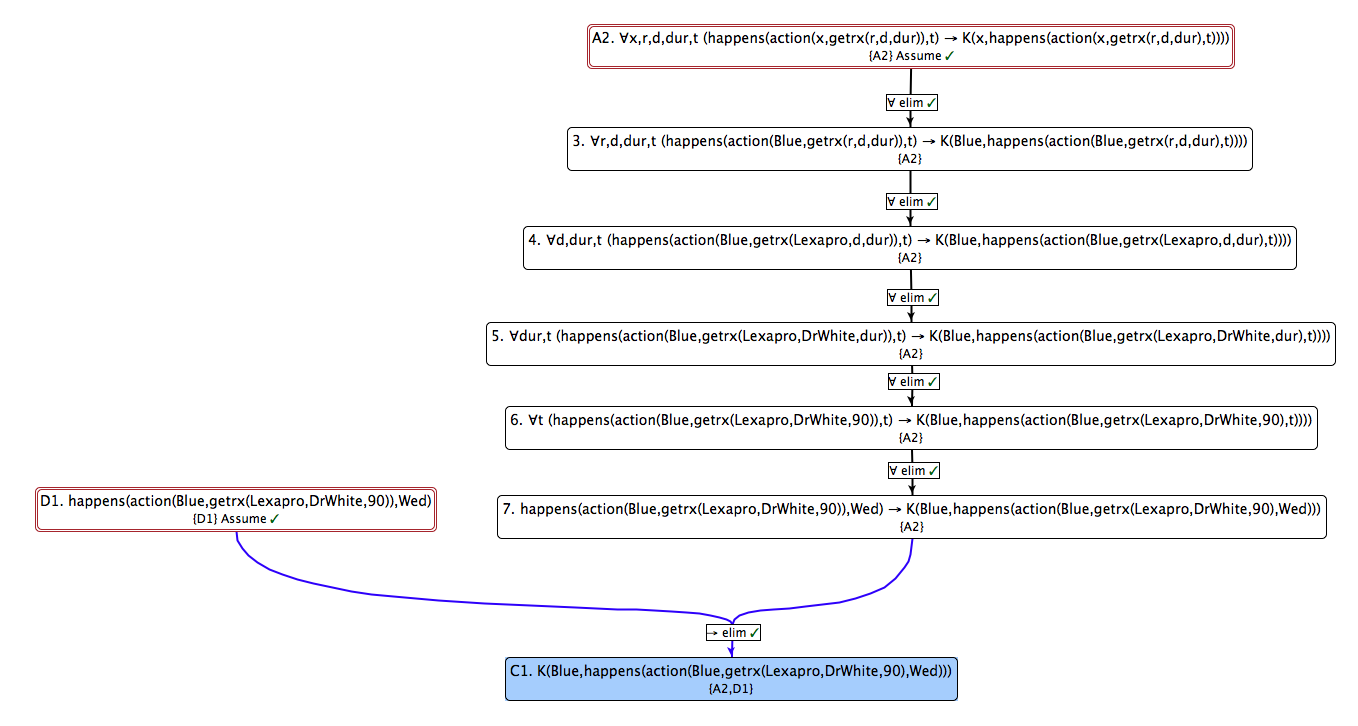
\includegraphics[width=1.0\textwidth]{c1_proof.png}}
\caption{Proof of $C1$ -- Blue knows he was given a prescription by Dr. White on 
Wednesday.}
\label{fig:proof_of_c1}
\end{figure}
%%++++++++++++++++++++++++++++++++++++++++++++++++++++++++++++++++++++

\noindent Next, the agent uses [$A2$] and [$D2$] to prove Blue also knows he was given a prescription by Dr. Black on Friday, as shown in Fig.~\ref{fig:proof_of_c2}, which stated formally, is as follows:
%% Conclusion2
%% Blue knows he gets a 90-day prescription for Lexapro from Dr. Black on Friday
\begin{footnotesize}
\begin{align*}
[C2] \ \knows(\Blue,\happens(\action(\Blue,\getrx(\Lexapro,\DrBlack,90)),\Friday))
\end{align*}
\end{footnotesize}

%%++++++++++++++++++++++++++++++++++++++++++++++++++++++++++++++++++++
\begin{figure}[h!] 
\vspace{6pt}
\centering
\framebox{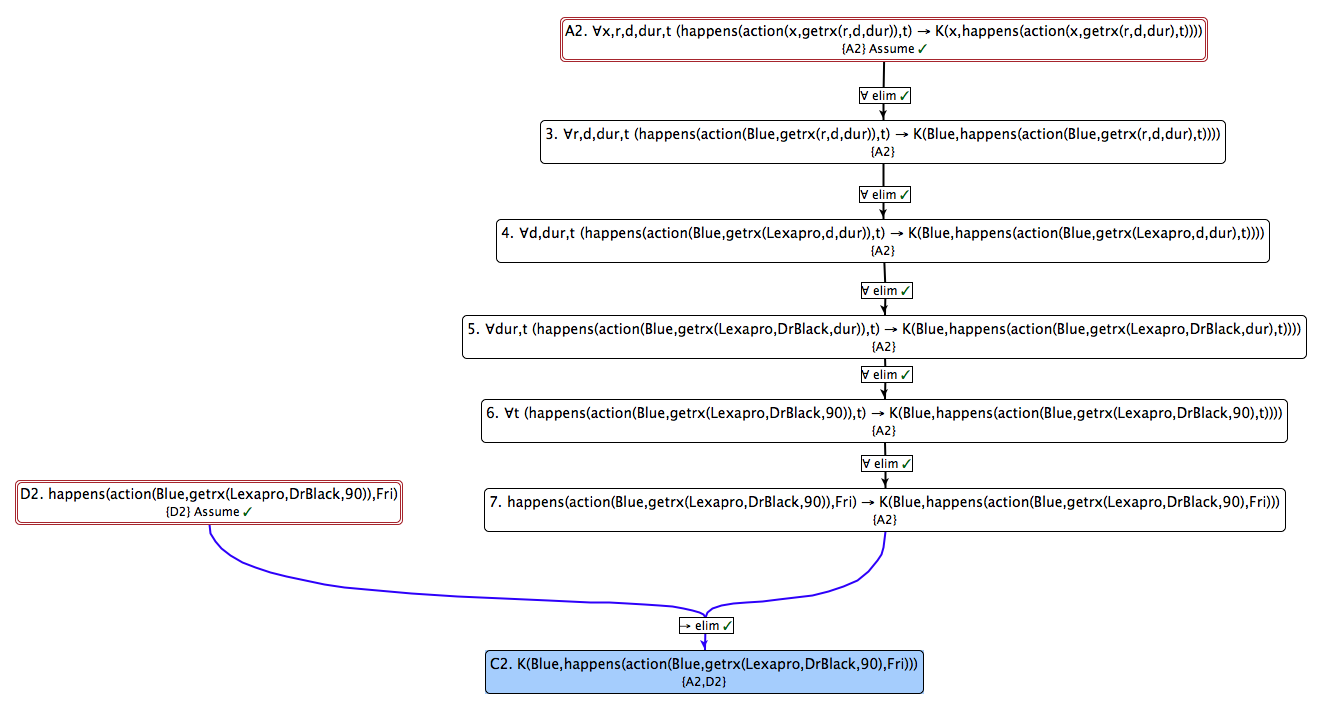
\includegraphics[width=1.0\textwidth]{c2_proof.png}}
\caption{Proof of $C2$ -- Blue knows he was given a prescription by Dr. Black on 
Friday.}
\label{fig:proof_of_c2}
\end{figure}
%%++++++++++++++++++++++++++++++++++++++++++++++++++++++++++++++++++++

\noindent Next, the agent uses [$A3$] to prove the conditional statement that if Blue does not tell Dr. Black about the prescription he received from Dr. White, then he \emph{knows} he does not tell him, stated formally in [C3] below.  The proof is shown in Fig.~\ref{fig:proof_of_c3}.

%% Conclusion3
%% If Blue doesn't tell Dr. Black on Friday that he received a prescription for 90 days Lexapro
%% from Dr. White on Wednesday, then he **knows** he didn't tell him this.
\begin{footnotesize}
\begin{align*}
[C3] \ \neg \happens&(\action(\Blue,\tells(\DrBlack,\\
& \happens(\action(\Blue,\getrx(\Lexapro,\DrWhite,90)),\Wednesday))),\Friday) \\
& \wedge \prior(\Wednesday,\Friday) \wedge \DrWhite \neq \DrBlack \Rightarrow \\
& \knows(\Blue, \neg \happens(\action(\Blue,\tells(\DrBlack,\\ 
& \happens(\action(\Blue,\getrx(\Lexapro,\DrWhite,90)),\Wednesday))),\Friday))
\end{align*}
\end{footnotesize}

%%++++++++++++++++++++++++++++++++++++++++++++++++++++++++++++++++++++
\begin{figure}[h!] 
\vspace{6pt}
\centering
\framebox{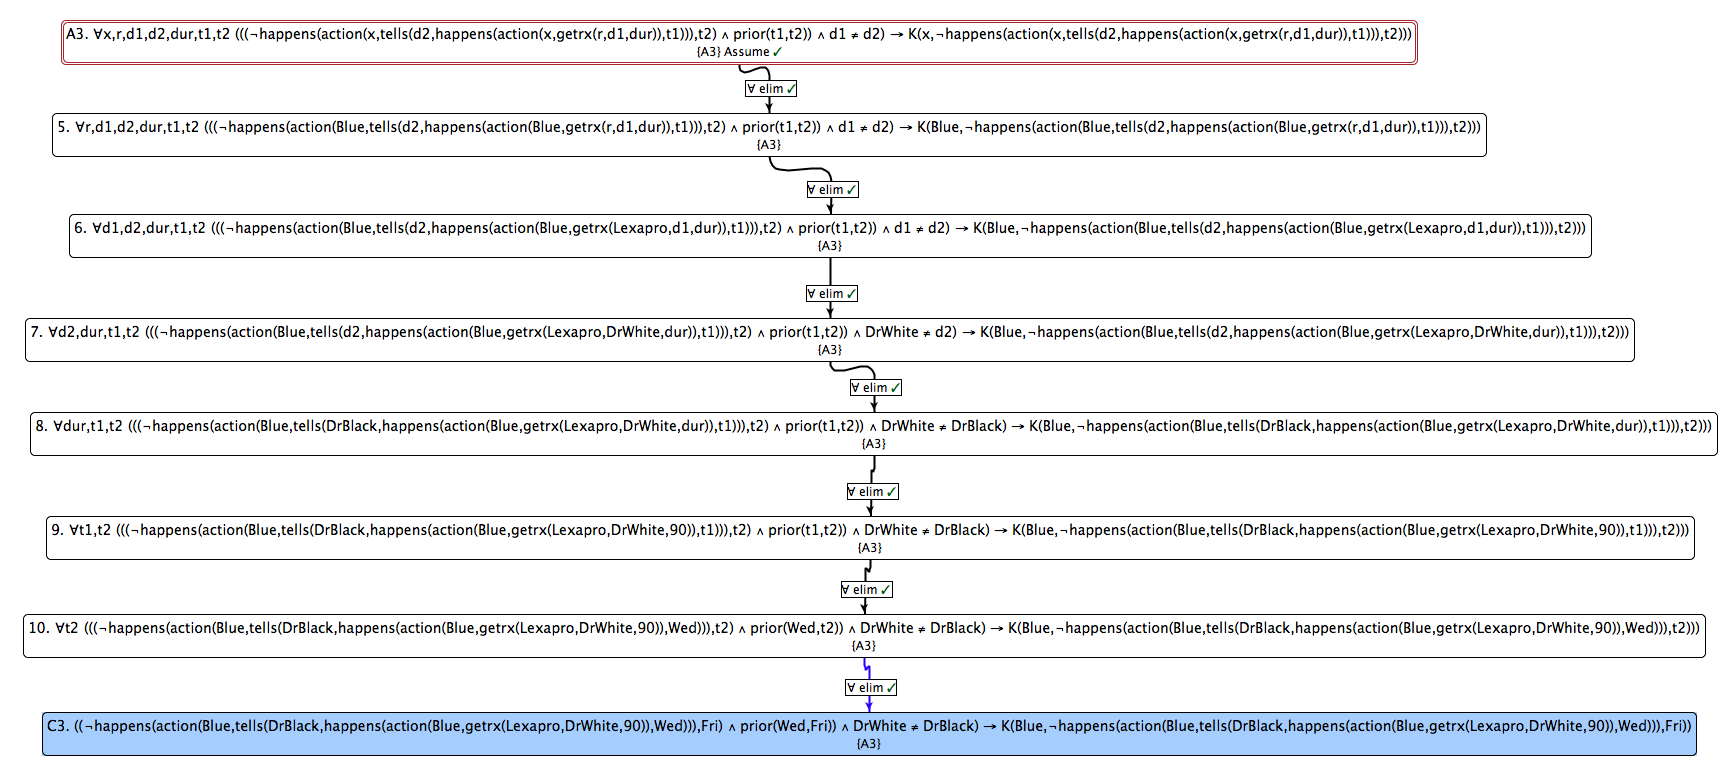
\includegraphics[width=1.0\textwidth]{c3_proof.png}}
\caption{Proof of $C3$ -- If Blue does not tell Dr. Black about the prescription he received from Dr. White then Blue knows he does not tell him.}
\label{fig:proof_of_c3}
\end{figure}
%%++++++++++++++++++++++++++++++++++++++++++++++++++++++++++++++++++++



\noindent Next, the agent uses [$C3$], [$D3$], and [$D4$] to prove the assertion that Blue believes that Dr. Black does not know about the fact he reeived a prescription from Dr. White on Wednesday, as represented formally by [$C4$], shown below.  This proof is shown in Fig.~\ref{fig:proof_of_c4}.  Also required by this proof are two supporting declations -- one about the order of occurence of Wednesday and Friday in a given week and another that asserts that $DrBlack$ and $DrWhite$ are constants referencing different objects (doctors, actually) in the problem domain.

%% Conclusion4
%% Blue believes Dr. Black does not know that Blue received a 90-day prescription for 
%% Lexapro on Wednesday
\begin{footnotesize}
\begin{align*}
[C4] \ \believes(\Blue, \neg \knows(\DrBlack,\happens(\action(\Blue,\getrx(\Lexapro,\DrWhite,90)),\Wednesday)))
\end{align*}
\end{footnotesize}

%%++++++++++++++++++++++++++++++++++++++++++++++++++++++++++++++++++++
\begin{figure}[h!] 
\vspace{6pt}
\centering
\framebox{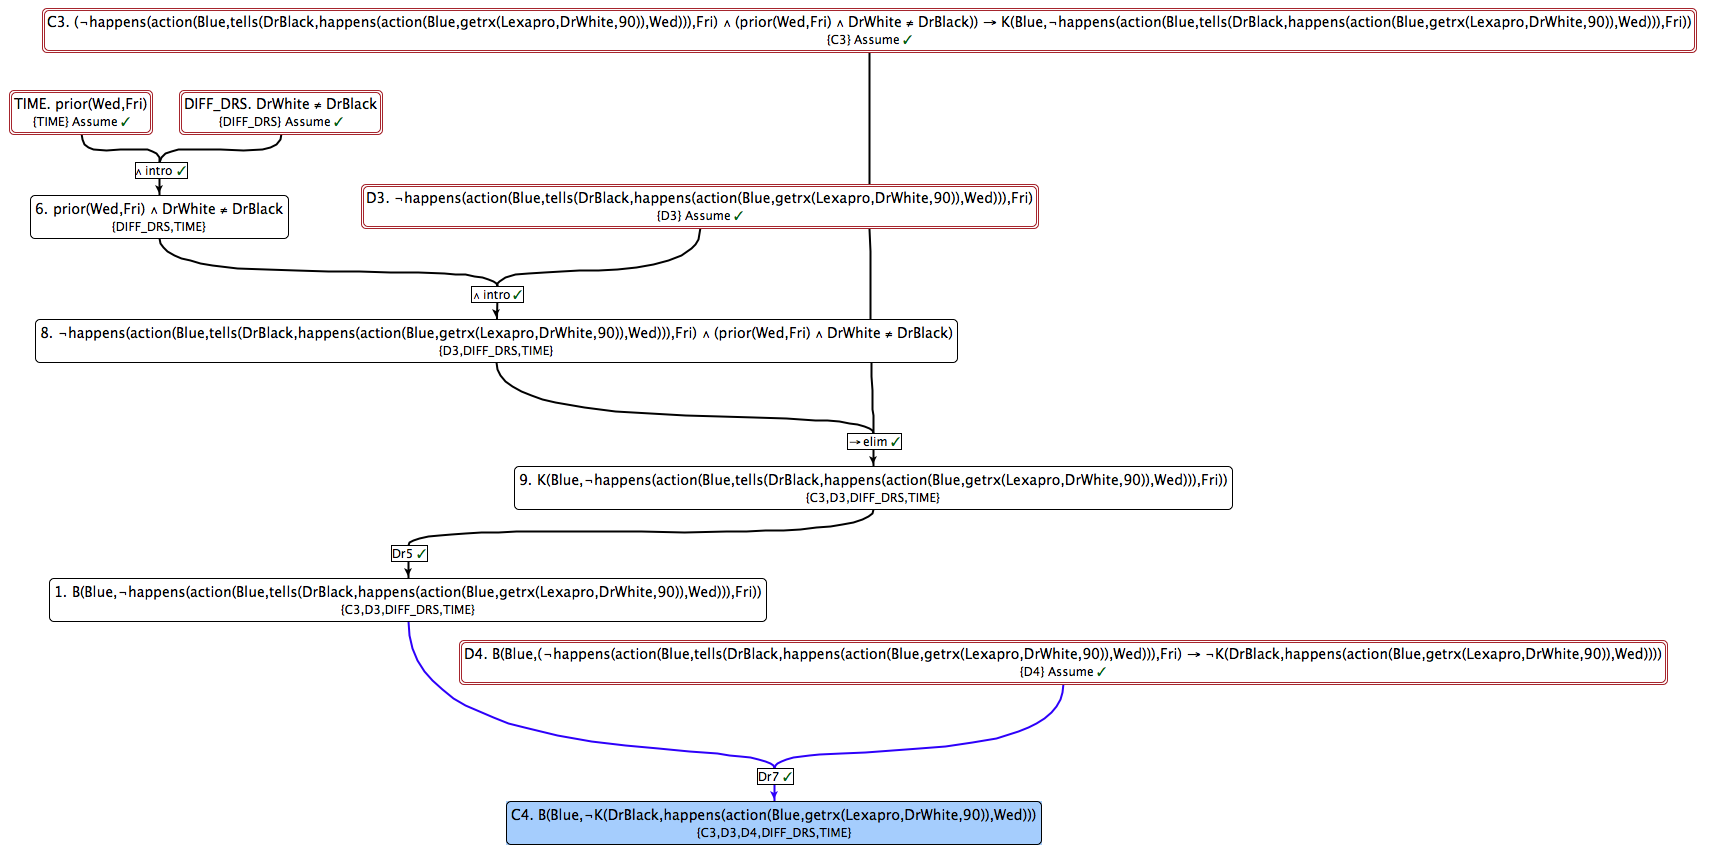
\includegraphics[width=1.0\textwidth]{c4_proof.png}}
\caption{Proof of $C4$ -- Blue believes that Dr. Black does not know he received a prescription from Dr. White on Wednesday.}
\label{fig:proof_of_c4}
\end{figure}
%%++++++++++++++++++++++++++++++++++++++++++++++++++++++++++++++++++++


\noindent Finally, using [$A1$], [$C1$], [$C2$], and [$C4$], the agent proves Blue is guilty of doctor shopping.  As was the case for the proof of [$C4$], the proof also requires supporting declarations related to time and the number of days between Wednesday and Friday relative to 10\% of the prescription duration.  This proof is shown in Fig.~\ref{fig:proof_of_c5}.
%% Conclusion5
%% Blue is guilty of doctor shopping.
\begin{footnotesize}
\begin{align*}
[C5] \ \guilty(\Blue,\Doctorshopping)
\end{align*}
\end{footnotesize}


%%++++++++++++++++++++++++++++++++++++++++++++++++++++++++++++++++++++
\begin{figure}[h!] 
\vspace{6pt}
\centering
\framebox{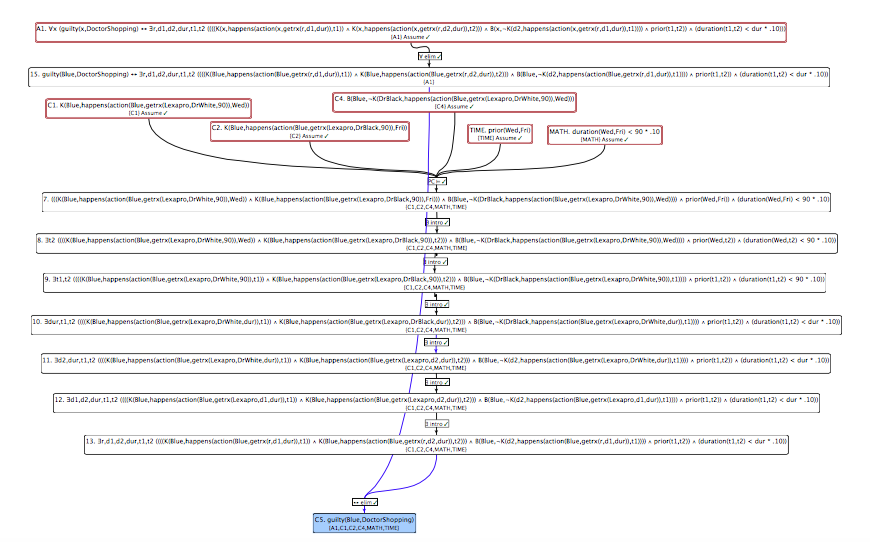
\includegraphics[width=1.0\textwidth]{c5_proof.png}}
\caption{Proof of $C5$ -- Blue is guilty of doctor shopping.}
\label{fig:proof_of_c5}
\end{figure}
%%++++++++++++++++++++++++++++++++++++++++++++++++++++++++++++++++++++

Taken together, these proofs add up to a completely transparent justification of the agent's reasoning for its ultimate conclusion that Blue is guilty of doctor shopping.  As mentioned earlier, this level of transparency is a feature of this formal, semantic approach that the approaches of Versions 1, 2, and 3 do not offer.  However, there are costs to this approach as well, as the reader may have noted during the walk-through of the proof.  First, natural language assertions must be translated into a formal language, as mentioned earlier.  And second, the model must be constructed such that it is comprehensive enough for the agent to make the necessary inferences it needs to complete the proof.  Niether of these is an easy task.  Often, assertions must be constructed based on common-sense-based real world knowledge, and are not explicitly stated in the text of supporting documentation or the scenario description.  Further discussion of these issues as well as the merits and pitfalls of the approaches we've seen to this point in the development of the CFE agent will be continued in Chapter 7.

This chapter adds another data point to our comparative analysis of state-of-the-art approaches to QA in terms of the competing priorities of accuracy, complexity, and reasoning justification.  In this case, the reasoning justification is higher than any of the approaches we've discussed, but comes at the cost of a great deal of complexity -- the issues in the preceding paragraph should be convincing on this point.


%% notes 06/09/2016

%1.  any formal definition of fraud must include the notion of intent.  It is not sufficient to define fraud in terms of a sequence of events in which resources are transferred from one party to another.  Fraud inherently involves the intent of one party to deceive another party for the purpose of gaining advantage or resources.  Intent 
%
%2.  intent implies knowledge.  thus, the definition in terms of cognitive states of fraud are steeped in assertions about knowledge.
%
%3.  if knowledge on the part of the suspected fraudster is not known, it is possible that the suspect simply engaged in a sequence of actions that might appear to be fraud but don't amount to fraud.  For example, what if, on the second attempt to procure an rx, the suspect, for whatever reason, was unaware that he already was given the rx.  For example, consider a situation in which the suspect gets a script for an rx, takes it home, but then loses it because his wife mistakenly throws it in the garbage.  Because he's traveling on business, he quickly goes to an out-of-town doctor who does not know the first doctor, and gets the same rx in order to replace the lost script.  This is clearly not fraud, but the fact that he goes to two doctors in quick succession to get the same rx would appear to be fraud.
%
%4.  However, how can a machine imbued with these extremely fine-grained definitions of fraud in relation to fine-grained mental states detect the mental states of all parties involved, most importantly the fraudster?  It can't.  Thus we need to make assumptions about mental states.  Specifically, we assume that the suspect, if he gets an rx, knows he's getting it, and doesn't forget that he got it when he gets the second one.  In other words, we assume the worst for the suspect, even though there are plausible circustances in which the suspect would not know, as discussed above.


%%\section{A First Example - The Law Related to Fraud 39}
%%
%%Fig.~\ref{fig:law_related_to_fraud_39_question} shows the first example we consider.  This question qualifies as a definition-type question, centering on the concept of larceny.  In order get this question correct, one must recognize that larceny is essentially synonymous with theft, or, pertinent to this question, stealing.  From this fact we make the following assertion regarding committing larceny in terms of stealing:
%%
%%\begin{footnotesize}
%%\begin{align*}
%%%%[A1] \ \forall t, a, x. \ & \happens(action(a, \bids(x+1), t+1)) \\ 
%%%%	& \Rightarrow \holds(highbid(x), t) \wedge \neg \holds(highbidder(a), t))
%%\end{align*}
%%\end{footnotesize}

%\begin{figure}
%\centering
%\vspace{1.0in}
%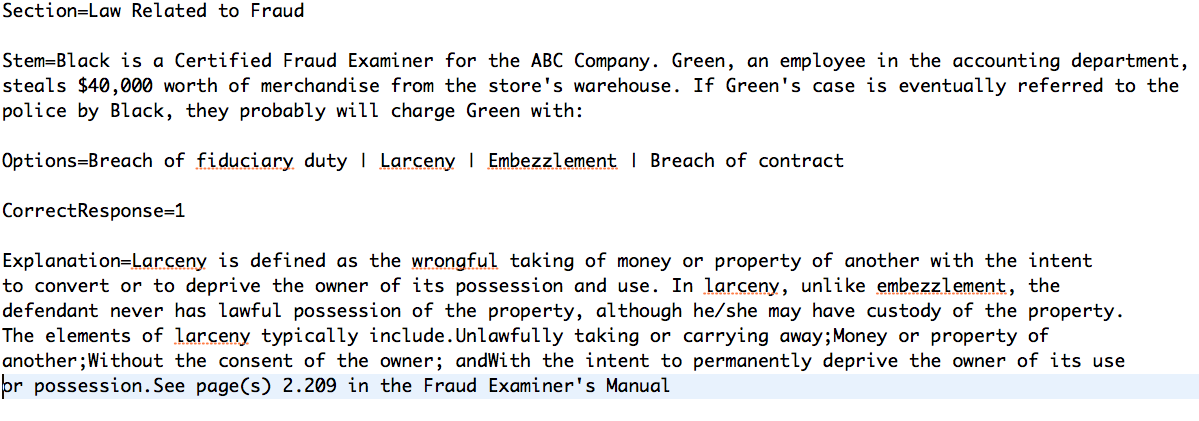
\includegraphics[width=100mm, height=50mm]{law_related_to_fraud_39_question.png}
%\caption{Law Related to Fraud 39}
%\label{fig:law_related_to_fraud_39_question}
%\end{figure}
%
%
%\begin{figure}
%\centering
%\vspace{1.0in}
%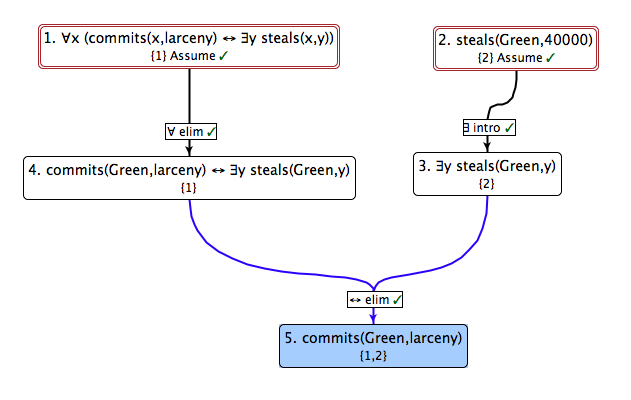
\includegraphics[width=50mm, height=60mm]{law_related_to_fraud_39_1.png}
%\caption{Law Related to Fraud 39 - Proof of Correct Answer (Larceny)}
%\label{fig:law_related_to_fraud_39_1}
%\end{figure}
%
%\begin{figure}
%\centering
%\vspace{1.0in}
%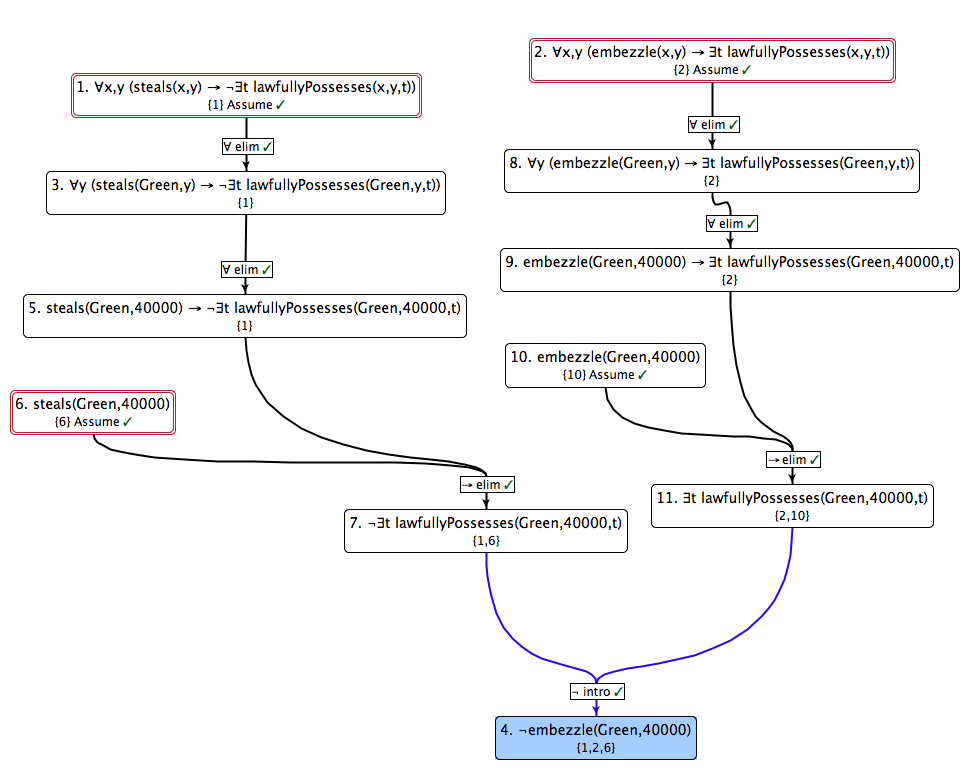
\includegraphics[width=50mm, height=100mm]{law_related_to_fraud_39_2.png}
%\caption{Law Related to Fraud 39 - Proof of Incorrect Answer (Embezzlement)}
%\label{fig:law_related_to_fraud_39_2}
%\end{figure}






















